\chapter{Methodology and Assumptions}
\label{chapter:methodology-and-assumptions}

In this thesis, an exploratory research method was used. The first reason is the qualitative nature of the three research questions. The second reason is the novelty of the interdisciplinary topics which have yet to be studied in depth. The exploratory research consists of the following steps:

\begin{enumerate}
	\item \textbf{Identifying Challenges and Creating a Hypothetical Solution --} Although precedence works have already identified challenges in each subtopic \seerefii{section:challenges-mechanical-challenges}{section:challenges-computational-and-design-challenges}, a holistic analysis is still needed as certain challenges that are coupled together \seeref{subsection:exploration-1-analysing-assembly-challenges}. This leads to a hypothetical robotic assembly process that is based on the idea of a robotic arm manipulating and collaborating with a set of robotic clamps \seeref{subsection:exploration-1-distributed-robotic-tool-approach}.

	\item \textbf{Testing, observing and refining the Hypothetical Solution --} Technical development is performed, and their behaviour is observed with empirical experiments. A number of iterations is performed to refine the hypothetical robotic assembly process and to better understand the problems involved \seeref{section:methodology-research-by-iterative-development}.

	\item \textbf{Formulating relationships --} Critical analysis is performed during the development in each iteration and at the end of the thesis to answer the research questions and to provide possible avenues for future in-depth studies \seeref{section:methodology-epistemological-assumptions}.

\end{enumerate}
\section{Research by Iterative Development}
\label{section:methodology-research-by-iterative-development}

The most important part of this exploratory research is the emphasis on system development and hands-on empirical trial runs to refine the hypothetical solution for automatic assembly. Five distinct development rounds were conducted, each containing their own research goals, technical developments, experiments and observations \seeref{subsection:methodology-setting-research-goals}. The flowchart in figure \ref{fig:thesis-exploration-flowchart} summarises the iterative process in the exploration rounds. 

\FloatBarrier
% 1 Image  
\begin{figure}[h]
    \centering
    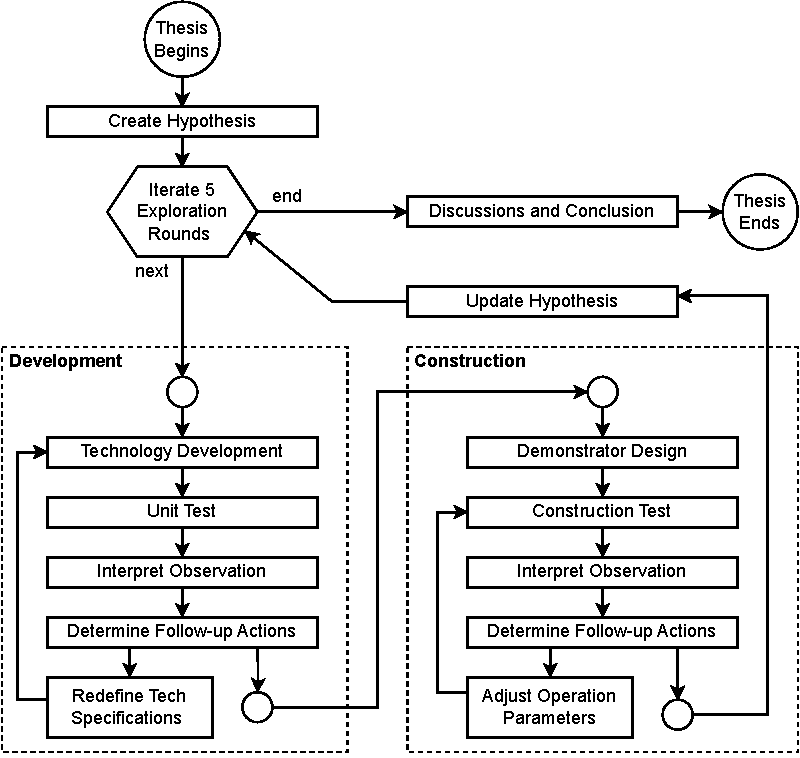
\includegraphics[width=0.99\textwidth]{images/03/Research by Iterative Exploration.pdf}
    \caption{Flowchart showing the iterative exploration research method}
    \label{fig:thesis-exploration-flowchart}
\end{figure}
\FloatBarrier

Within each \textbf{Development Phase}, small scale tests were performed and the technology was improved until it was ready for a full systematic test \seeref{subsection:methodology-technology-development}. 

The full systematic test was performed by designing and constructing a \textbf{Demonstrator Structure} \seeref{subsection:methodology-demonstraror-design}. 

During the \textbf{Construction Phase}, certain adjustments of the process parameters are also possible. Afterwhich, the follow-up actions are determined for the next exploration round \seeref{subsection:methodology-observations-and-interpretation}.

\subsection{Setting Research Goals}
\label{subsection:methodology-setting-research-goals}

At the beginning of the first iteration, the goal was to design and prototype an assembly process and to test it with experiments. As new insights and discoveries are made, subsequent development iterations are guided by the discoveries and include follow-up explorations whenever necessary. Below is a summary of the goals in each phase:

\newcommand{\explorationbullet}{\raisebox{.10ex}{\large$\bullet$}}

\begin{description}[style=standard] % Environment provided enumitem package

    \item [Exploration Round 1 - Clamp Prototype] A minimal demonstration of the robotic clamp concept is developed to verify the process. The hardware being developed is only capable of assembling one type of lap joints with fixed dimensions. Nevertheless, it successfully performed the task and revealed opportunities for further improvements. \seeref{chapter:exploration-round-1}
    
    \item [Exploration Round 2 - Bus Stop Demonstrator] The initial proof-of-concept clamp is redesigned to accommodate joints with different angles. Software is also developed to generate robot trajectory, control the robot arm, and control the robotic clamps wirelessly. Finally, a high level controller is developed to synchronise motion between the robotic arm and robotic clamps - an important aspect of the assembly process. The entire system was validated through the construction of a timber frame structure with 40 elements. \seeref{chapter:exploration-round-2}
    
    \item [Exploration Round 3 - Automatic Clamp Placement] This phase completes the automation for mechanical tasks that are identified as low priority in the previous two phases. One of the highlights is the automatic placement and retrieval of robotic clamps on the structure. In addition, task planning and motion planning algorithms were introduced to study the automation of parsing designs to create robotic assembly programmes. The completed fully automatic assembly system was validated by reassembling the last demonstrator in a fully automatic manner. \seeref{chapter:exploration-round-3}
 
    \item [Exploration Round 4 - HyparHut Demonstrator] This phase consists of a UI upgrade to improve interactive modelling in the CAD environment, the introduction of a fabrication-aware design workflow, and the introduction of a new robotic screwdriver. The new screwdriver allows the assembly of non-planar lap joints and can accommodate timber beams with different profile sizes. This vastly expands the design possibilities for timber frame structures that can be assembled by the automatic process. The new system was validated with the assembly of a structure with a hyperbolic paraboloid roof. One other highlight was the introduction of a vision based alignment process for improving the success rate for the robotic arm to pick up and place tools. \seeref{chapter:exploration-round-4}
    
    \item [Exploration Round 5 - CantiBox Demonstrator] By this round, the robotic assembly process had already achieved a high degree of automation and required little human intervention. The study was therefore expanded to integrate cutting-edge design methods with collaborators in two different fields. The first is structurally-informed joint design using novel design methods that is based on the theory of plasticity. This allows individually customised joints to respond to local load conditions. The main challenge on my part was to negotiate the intersection between assembly limitations, Computer Numeric Control (CNC) machining limitations and structural optimization. The second is automated Task and Motion Planning (TAMP) using PDDLStream to optimise redundant tasks and robotic motions. The main challenge is to formulate actions that can be understood by the computer algorithm to plan automatically. The combined technology was validated with the assembly of a structure with three modular boxes, each containing clamped and screwed joints. This also saw the largest amount of tools being used by the robotic assembly process, which provided insight for the future of the system. \seeref{chapter:exploration-round-5}
 
\end{description}
\subsection{Technology Development}
\label{subsection:methodology-technology-development}

The robotic assembly process required the development of novel hardware and software that form systems and subsystems that are interdependent in their operations. Below is an overview of the development categories showing their multidisciplinary nature. The software tools that are used for their development are listed in the bracket. 

\begin{description}[nosep]
	\item \textbf{Mechatronics Design}
    \begin{itemize}
    	\item Robotic arm attachment hardware design (Rhinoceros 3D) 
    	\item Robotic clamp and screwdriver hardware design (Rhinoceros 3D) 
    	\item Robotic clamp and screwdriver drive electronics design (EAGLE)
    	\item Other static hardware supporting construction (Rhinoceros 3D) 
    \end{itemize}
    
	\item \textbf{Software for Computer-Aided-Design (CAD)}
    \begin{itemize}
    	\item CAD library for modelling timber parts and their assembly (Python)
    	\item Design validation tools (Python)
    	\item User Interface (UI) for interactive design modelling and validation (Python in Rhinoceros 3D) 
    	\item CAM library for modelling robotic tools and their actions (Python)
    \end{itemize}
    
    \item \textbf{Software for Computer-Aided-Manufacturing (CAM)}
    \begin{itemize}
    	\item Interface with Task and Motion Planning (TAMP) software (Python)\footnote{In collaboration with YiJiang Huang (MIT)}
    \end{itemize}
    
    \item \textbf{Software for control and execution}
    \begin{itemize}
    	\item Robotic clamp and screwdriver firmware (C++)
    	\item Wireless communication firmware (C++)
    	\item Robotic arm and robotic tools synchronisation controller (Python, ROS)
    	\item Task execution and process monitoring software (Python)
    \end{itemize}
\end{description}

During development, multiple technical solutions can often be used to achieve a particular goal. The principle for selecting a specific option included the following criteria: 

\begin{enumerate}[nosep]
	\item The cost of implementation is reasonable in the architectural construction context, and testing costs can be afforded by the given research budget.
	\item The implementation can be tested and observed within our laboratory.
	\item Software and hardware dependency is open source.
	\item The implementation is potentially generalisable (e.g. a tool that can assemble more types of joints).
	\item The implementation is compatible with existing industrial practices or norms (e.g. working with existing construction-grade tolerance instead of demanding a car-component-like accuracy).
\end{enumerate}

Given the complexity of the AEC industry and its tendency to resist systematic changes, these principles guided the research direction towards finding implementable solutions with high impact.

\subsection{Demonstrator Design}
\label{subsection:methodology-demonstraror-design}

At the end of development phase 2, 4 and 5, the developed assembly process was observed and evaluated by the construction of a prototype structure. This is often called a demonstrator in the field of digital fabrication research. In total, there were three real-scale (1-to-1) demonstrators designed for this thesis. For the purpose of technical evaluation, the use of real-scale experiments revealed issues that were otherwise not observable in a computer simulation or a small-scale test. From the perspective of architectural design, the demonstrators served as a design study that can be experienced in person. Because of the high material cost and long preparation time required to construct such a demonstrator, each of them serves multiple investigation purposes to maximise the knowledge that can be extracted. Below is a list of design guidelines used when designing the demonstrators:

\begin{enumerate}[nosep]
	\item The structure can be constructed with the developed system.
	\item The structure fits within our laboratory.
	\item The structure can demonstrate the flexibility of the assembly system (e.g. different types of joints, different joint angles, different element sizes, and different numbers of elements).
	\item The structures should present various difficulties for the assembly system (e.g. assembling very long elements, reaching into a congested space, joints very close to the ground or very high, many simultaneously assembled joints).
	\item The structures should contain various types of load-bearing elements (e.g. columns, floor beams, joists, diagonal bracings, rafters).

\end{enumerate}
During the design and preparation of the demonstrator, the newly developed CAD software (data structures, algorithms and user interfaces) was observed when it was used to model and encode the design. Flexibility and usability was observed first hand by the author, and improvements are sometimes implemented within the same development phase. The CAM software for translating design to robotic trajectories and execution programs was also tested. The result of this software is validated by performing digital checks such as robot kinematic simulation to catch collision problems. These problems must be fixed before the design phase can be concluded and timber parts can be ordered from the fabricator. 

During the demonstrator construction (also called Robotic Execution), the mechatronics hardware and control software was observed. The observation includes the dynamic behaviour when assembling different joint geometry and beam sizes at different orientations and with different support conditions. These observations provided evidence to identify key factors that limit system performance.  In addition, real world effects (such as gravity, material and robot inaccuracy) were observed during the assembly process to better understand fabrication constraints. This was used to improve the accuracy of automatic design checks for the fabrication-aware workflow. Finally, unplanned manual interventions, such as robotic collisions, and overload errors due to jamming, are recorded and analysed qualitatively to identify patterns.

The timber parts used for the demonstrators were ordered from an industrial timber fabricator. Ordering from industry was preferred over creating the components within our laboratories because it allows a reality check of whether the newly developed digital workflow and timber details are compatible with the existing upstream industry. A single company (Auer Holzbau, Switzerland) was used to provide all the machining services in favour of consistency. The machining was performed on a recently released automatic joinery machine model (ROBOT-Drive 1250) manufactured by Hans Hundegger AG, Germany. The transfer of timber geometrical data is based on a proprietary file format of Cadwork (version 28). This is because the timber machining industry in Switzerland accepts it as a de facto standard for contractual agreement on the geometry of parts.

\subsection{Observations and Interpretation}
\label{subsection:methodology-observations-and-interpretation}

The \textbf{observations }made during the preparation and the execution of the demonstrators are documented as objectively as possible for each development phase (from Chapters \ref{chapter:exploration-round-1} to \ref{chapter:exploration-round-5}). 


% 1 Image  
\begin{figure}[ht]
    \centering
    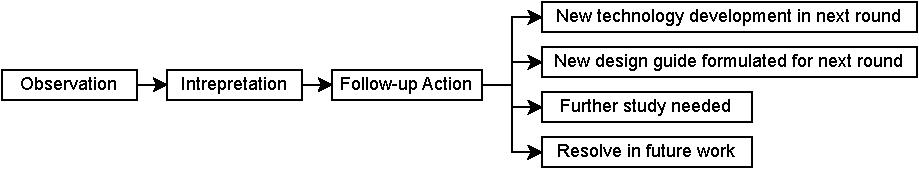
\includegraphics[width=0.99\textwidth]{images/03/Observation to followup actions.pdf}
    \caption{Workflow from observation to interpretation and follow-up actions}
    \label{fig:observation_andinterpretation_workflow}
\end{figure}


Based on these observations, \textbf{interpretations }are made to explain success and failure and are subsequently used to determine \textbf{follow-up actions}. Readers should be aware of the possible subjectivity in the interpretations and follow-up actions \seerefii{section:methodology-epistemological-assumptions}{section:methodology-axiological-assumptions}. 

Figure \ref{fig:observation_andinterpretation_workflow} shows different types of follow-up actions. For example, an observation may suggest new technology developments to improve the robotic assembly system. In some cases, further studies may be necessary to verify a causal relationship where the interpretations may be inconclusive. This can be caused by the scarcity of observations or the lack of scientific controls. Some other problems may require a design solution rather than a technological one, which can be addressed by formulating design guidelines or by creating automatic design checks. 

Note that some of the follow-up actions, such as adjusting software and tuning operation parameters, can be performed within the same exploration round. On the other hand, during the construction phase, the prefabricated timber parts cannot be modified easily and issues related to the demonstrator design can only be addressed in the next iteration. In addition, mechatronic and hardware issues often require substantially longer time to resolve. These problems were mostly addressed in the next round. 

Finally, follow-up actions are implemented wherever appropriate as long as my skills, research time and budget allow. Otherwise, the problems are elaborated for future investigations. 

\section{Epistemological assumptions}
\label{section:methodology-epistemological-assumptions}

The aim of the research is to create knowledge by developing, integrating and observing the effects of various technologies and the decisions made when designing the demonstration structure.

\textbf{Success and Failure} were evaluated based on whether the observed technology supports the vision of automatic design-to-assembly for timber frame structures. While some of the evaluation metrics are quantitative, others are qualitative such as when studying the generalizability and limitations of a particular technology.

\textbf{Causal Relationships} were established by logical reasoning, discussion with domain experts (e.g. CNC operator, Robot Technician, Structural Engineer, Architect) or quantitative experiments (e.g. tuning operation parameters, substituting parts or subsystems). The specific method to identify relationships was selected individually depending on the nature of the inquiry.

\section{Axiological assumptions}
\label{section:methodology-axiological-assumptions}

This thesis followed interpretivism principles, and many of this research's components are qualitatively analysed. Readers should therefore be aware of the author’s (my) background and its potential influence on the interpretation of data. In the rest of the thesis, first-person pronouns (i.e. I, my) are used as an indication of when decisions and interpretations are likely to be influenced by my background. Passive voice will continue to be used to describe objective observations and when making qualitative analyses.

\subsection{Researcher Background}
\label{subsection:methodology-researcher-background}

I was trained at the undergraduate and graduate levels as an architectural designer specialising in computational design. I have also practised mechatronics design in art and design, albeit without formal training. These experiences greatly influence my characterisation of the research questions as a technology development problem focusing on mechatronics and computational design instead of other pathways. For example, another researcher with a timber engineering background may approach the problem by proposing novel wood joints, or a roboticist may propose a novel control method for robotic manipulators. Nevertheless, mechatronics and computational design are the most common approach taken by many recent research projects, as introduced in the previous chapters.

\subsection{Laboratory Context}
\label{subsection:methodology-laboratory-context}

The research is conducted in the Robotic Fabrication Lab (RFL) of the Institute of Technology in Architecture (ITA) at the Department of Architecture of ETH Zurich, where four industrial robotic arms are mounted upside-down on two gantry robots (custom design by Güdel Group AG, Switzerland), forming a robotic manipulator that covers a large space \seeref{subsection:exploration-2-rfl-robotic-platform}. Each robot consists of six articulated joints, an independent vertical linear axis, and two horizontal linear axes on the gantry coupled with neighbouring robots. If only a single robot is concerned, all nine axes can be commanded to move synchronously. This offers kinematic redundancy that allows the robot body to avoid obstacles in dense environments. For this thesis, the robotic manipulator in the RFL represents a hypothetical robotic manipulator that acted as a testbed for developing the robotic assembly process. This also carries the assumption that lessons learnt from this setup can be extrapolated to on-site setups in the future. The details of this extrapolation are further discussed in the conclusion chapter \seeref{subsection:extrapolation-to-on-site-robots}. 

Our laboratory is also the home to many timber assembly research projects introduced in the context. This undoubtedly influences the research as existing robotic components and software infrastructure are adopted from previous research. For example, the choice of the automatic robotic quick-change system was the result of a donation from previous projects \seeref{subsection:exploration-2-docking-adapter}. Another example is the choice of online robot control middleware \seeref{subsection:exploration-2-distributed-control-system}, which was determined by our laboratory's standard mode of operations.

\subsection{Participants in User Interface Study}
\label{subsection:methodology-participants-in-user-interface-study}

While the user interface consists of only a small portion of the development work, it is interesting to observe how designers can use the newly developed design interface. In order to gather a bigger picture, participants (other than myself) are invited to design two of the three demonstrators. During the design sessions, which often span multiple weeks, I offered technical guidance to the designer and observed what knowledge I explicitly communicated to the participant. This mitigates some of my subjectivity when considering implicit versus explicit knowledge, especially because I am the main developer of both software and hardware systems. 

\section{Collaborations}
\label{section:methodology-collaborations}

Throughout this thesis, I collaborated with domain experts for some technological developments outside of my skills and knowledge. Their expert knowledge about state of the art in their respective fields helped me formulate the initial hypothetical solution. 

\begin{itemize}
	\item \textbf{Structural Analysis and Timber Joint Design }problems were advised by Dr. Davide Tanadini (Chair of Structural Design, ETH Zurich). His research focuses on possible applications of the theory of plasticity and graphic statics on timber structures and joints and their implementation in digital fabrication. In particular, the last demonstrator was designed by a student under his supervision (global design) and the joints were customised by the models and software he developed as part of this thesis. His PhD dissertation is titled ``Limit analysis and timber plasticity. Plastic design of interlocking timber-to-timber connections" \parencite{tanadiniLimitAnalysisTimber2023} Together with this thesis, they form part of the NCCR Digital Fabrication research project ‘Spatial Timber Assemblies’.

	\item \textbf{Robotic Task and Motion Planning (TAMP) }problems were advised by Dr. Yijiang Huang (Digital Structures Research Group, MIT, USA). His introduction and advice to the field was essential for me to understand the nature of the complicated problems involved. We worked in close collaboration for realising the three demonstrators, which led to the discovery of many new techniques to bridge between the highly technical fields (robotics and computer algorithms) and architectural design. Many of the planning related software, including all of the motion planning backend were developed by him. His PhD dissertation is titled ``Algorithmic planning for robotic assembly of building structures," \parencite{huangAlgorithmicPlanningRobotic2022}. Both of our researches share the same vision towards improving automation from design to assembly. 

	\item \textbf{Machine Design and Construction}, especially the later development with the screwdriver were advised by Prof. Dr. Agathe Koller and Marco Rossi (both from The Institute for Lab Automation and Mechatronics ILT, OST, Switzerland). They were directly involved in the conceptualization of the screwdriver operation mechanism and the innovative pin gripper mechanism. Marco also offered valuable instructions for machine design and construction, made some of the hardware parts and advised on the tests during hardware development

\end{itemize}
\section{Thematic Reading Guide}
\label{section:methodology-thematic-reading-guide}

The following five chapters (chapter 4 to 8) are written in chronological order corresponding to five development rounds. This is important for understanding the exploration as an evolution between experiments and observations.  Each chapter contains the following sections:

\begin{description}
	\item [1. Goal] Identify the goal and scope for the entire exploration round.
	\item [2. Background] Background knowledge needed to understand the rationale for some of the development.
	\item [3. Development] Technical description of the developed hardware and software. Some topics include the tests that were performed during development.	
    \item [4. Demonstration] Systematic test was performed by designing and constructing a demonstrator structure.
	\item [5. Lesson Learnt] Observations, findings and interpretations related to the robotic construction demonstration. Some topics include hypotheses of possible cause(s), possible solution(s) and the follow-up action(s) taken. 
\end{description}

Readers who are interested only in a specific theme may find the following guide helpful for identifying a specific section. Note that this list is not exhaustive. 

\begin{itemize}

	\item \textbf{Distribute Robotic Tools (DiRT) assembly method}

    \begin{itemize}
    	\item \textbf{Initial working hypothesis} of the DiRT clamps assembly method \seeref{subsection:exploration-1-dirt-clamping-assembly-process-task-list-v1}
    
    	\item \textbf{Operation method revised} after initial test \seeref{subsection:exploration-3-dirt-clamping-assembly-process-task-list-v2}
    
    	\item \textbf{Operation method with screwdrivers} \seeref{subsection:exploration-4-flowchart-for-screwdriver-assembly}
    
    	\item \textbf{Operation method with clamps and screwdrivers }\seeref{subsection:exploration-5-combined-operation-of-clamps-and-screwdrivers}
    
    	\item \textbf{Generalised operation principle} \seeref{section:discussion-generalised-dirt-system}
    
    \end{itemize}
	\item \textbf{Two Types of DiRT Assembly Tools}

    \begin{itemize}

        \item \textbf{Clamp }for planar lap joints

        \begin{itemize}[nosep]
        	\item Hardware \seeref{subsection:exploration-2-lap-clamp-cl3-hardware}
        	\item Electronics \seeref{subsection:exploration-2-cl3-clamp-electronics}
        	\item Firmware \seeref{subsection:exploration-2-cl3-firmware}
        \end{itemize}
        \item \textbf{Screwdriver }for planar and non-planar lap joints 

        \begin{itemize}[nosep]
        	\item Hardware \seeref{subsection:exploration-4-lap-screwdriver-sl1-and-sl1-g200-hardware}
        	\item Electronics \seeref{subsection:exploration-4-sl1-screwdriver-electronics}
        	\item Firmware \seeref{subsection:exploration-4-screwdriver-firmware-l1-control}
        \end{itemize}
    \end{itemize}
	\item \textbf{Other DiRT supporting hardware}

\begin{itemize}
	\item \textbf{Radio} \seeref{subsection:exploration-2-radio-network}

	\item \textbf{Gripper}

\begin{itemize}[nosep]
	\item Short Parallel Gripper \seeref{subsection:exploration-2-parallel-gripper-pg500-and-pg1000}

	\item Long Parallel Gripper \seeref{subsection:exploration-4-parallel-gripper-pg1500-for-long-beams}

	\item Pin Gripper on Screwdriver \seeref{subsection:exploration-4-pin-gripper-mechanism}

\end{itemize}
	\item \textbf{Docking Adapter}

\begin{itemize}
	\item Docking Sensor \seeref{subsection:exploration-4-docking-adapter-lock-sensor}

\end{itemize}
	\item \textbf{Camera Alignment System}

        \begin{itemize}[nosep]
        	\item Alignment and Correction Concept \seeref{subsection:exploration-4-camera-marker-alignment-correction-system}
        	\item Camera on Docking Adapter \seeref{subsection:exploration-4-camera-marker-hardware-on-docking-adapter}
        	\item Camera on CL3 Clamp \seeref{subsection:exploration-5-camera-marker-hardware-on-cl3-clamp}
        	\item Docking Process \seeref{subsubsection:exploration-4-visual-guided-docking-process}
        
        \end{itemize}
\end{itemize}
	\item \textbf{Design Software and Workflow}

    \begin{itemize}
    	\item \textbf{Design and Modeling Frontend}
    
        \begin{itemize}[nosep]
        	\item \textbf{Design UI in Rhino Grasshopper} \seeref{subsection:exploration-2-cad-cam-user-interface}
        	\item \textbf{Design UI (revised) in Rhino Python } \seeref{subsection:exploration-3-design-software-implementation-in-rhino-python}
        	\item \textbf{Process Design Visualization} \seeref{subsubsection:exploration-3-process-visualization-and-adjustment}
        \end{itemize}
        
    	\item \textbf{Backend}
        \begin{itemize}[nosep]
            \item \textbf{Assembly Model} \seeref{subsection:exploration-2-assembly-model-data-structure-and-functions}
            \item \textbf{Process Model} \seeref{subsection:exploration-3-process-design-workflow}
        \end{itemize}
        
    	\item \textbf{Conceptual}
        \begin{itemize}[nosep]
        	\item Deformation Awareness and Error Correction \seeref{subsection:exploration-4-deformation-awareness-and-error-correction-by-triangulation}
        	\item Global Error Correction \seeref{subsubsection:exploration-4-global-correction-approach}
        \end{itemize}
    \end{itemize}

	\item \textbf{Task and Motion Planning Workflow} \seeref{subsection:exploration-3-process-design-workflow}

    \begin{itemize}
    	\item \textbf{Narrow Passage Problem } \seeref{subsection:exploration-2-narrow-passage-problem}
    
    	\item \textbf{Fast Check by IK} \seeref{subsection:exploration-4-fast-design-validation-with-ik-check}
    
    	\item \textbf{Fast Check by LMG Planning} \seeref{subsection:exploration-4-planning-order-by-motion-group}
    
    	\item \textbf{Non-sequential MMMP Solver} \seeref{subsection:exploration-3-taught-configuration-for-repetitive-targets}
    
    \end{itemize}
	\item \textbf{Three Demonstration Structures Constructed}

\begin{itemize}[nosep]
	\item \textbf{BusStop Pavilion} \seeref{subsection:exploration-2-demonstrator-design-busstop-pavilion}

	\item \textbf{HyparHut Pavilion} \seeref{subsection:exploration-4-demonstrator-design-hyparhut-pavilion}

	\item \textbf{CantiBox Pavilion} \seeref{subsection:exploration-5-demonstrator-design-cantibox-pavilion}

\end{itemize}
\end{itemize}
